% command to make sure colorboxes don't create whitespace between code lines
\fboxsep=.6pt

% default settings for listings
\lstset{style=python}

\title[Daten Vorhersagen]{Daten Vorhersagen: Korrelation \& Kausalität}

\subtitle{Mehrere Bedingungen verbinden}

\author[Wendl, Cyril] % (optional)
{Cyril Wendl \inst{1}}

\institute[KLW] % (optional)
{
    \inst{1}%
    Fachschaft Informatik\\
    Kantonsschule im Lee
}

\date[\today] % (optional)

\logo{\includegraphics[width=2cm]{\thelogo}}

\titlegraphic{\vspace{-.7cm}\includegraphics[width=\textwidth]{"GrundlagenInfo/06_Datenbanken/Figures/title-emojis"}}

\frame{\titlepage}
\begin{frame}{Korrelation \& Kausalität: Polizeipatrouillen und Straftaten}
    \begin{figure}[H]
        \centering
        \includegraphics[width=0.7\linewidth]{"GrundlagenInfo/10_AusDatenLernen/Figures/polizei_vs_kriminalitaet"}
        \caption{Anzahl Polizeipatrouillen und begangene Straftaten}
        \label{fig:polizei_vs_kriminalitaet}
    \end{figure}
\end{frame}

\begin{frame}{Korrelation \& Kausalität: Social-Media-Nutzung und Zufriedenheit}
    \begin{figure}[H]
        \centering
        \includegraphics[width=0.7\linewidth]{"GrundlagenInfo/10_AusDatenLernen/Figures/socialmedia_vs_zufriedenheit"}
        \caption{Social-Media-Nutzung und Zufriedenheit}
        \label{fig:socialmedia_vs_zufriedenheit}
    \end{figure}
\end{frame}
    

\begin{frame}[fragile]{Ziele der heutigen Lektion}
    Ziele
        \begin{enumerate}[<+->]
            \item \faCheckSquare{} Ich kann den Unterschied zwischen Korrelation und Kausalität erklären.
            \item \faCheckSquare{} Ich kann begründete Einschätzungen über die Kausationsart zwischen zwei Variablen abgeben, indem ich folgende Begriffe verwende:
            \begin{itemize}
                \item \faCheckSquare{} Koinzidenz
                \item \faCheckSquare{} Zyklische Beeinflussung
                \item \faCheckSquare{} Gemeinsamer Grund
                \item \faCheckSquare{} Indirekte Kausalität
                \item \faCheckSquare{} Direkte Kausalität
            \end{itemize}
            \item \faCheckSquare{} Ich wende bei der Interpretation von korrelierten Daten Vorsicht an, bevor ich Aussagen über Kausalität treffe.
            \item \faCheckSquare{} Ich kann die Zahl \( Z \) berechnen und interpretieren.
        \end{enumerate}
\end{frame}


\begin{frame}{Definition: Kausalität}
    \begin{mydefinition}[Kausalität]\label{def:kausalitaet}
        \textbf{Kausalität} beschreibt eine Ursache-Wirkung-Beziehung zwischen zwei Variablen, welche wir im Allgemeinen A und B nennen. Wenn eine Variable A (Ursache) eine andere Variable B (Wirkung) beeinflusst, spricht man in diesem Fall von Kausalität. Um zu beurteilen, ob eine Kausalität vorliegt, ist es wichtig, den Zusammenhang zwischen den Variablen zu analysieren und zu verstehen. Kausalität kann häufig nur durch wissenschaftliche Experimente oder statistische Analysen nachgewiesen werden. Kausalität ist ein sehr komplexes Thema und es gibt viele verschiedene Arten von Kausalität.
    \end{mydefinition}
\end{frame}

\begin{frame}{Arten von Kausalität: Koinzidenz}
    \textbf{Koinzidenz} beschreibt eine zufällige Korrelation zwischen zwei Variablen, die keine kausale Beziehung haben.
    \begin{center}
        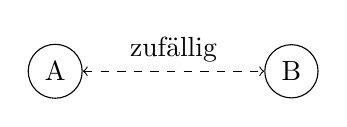
\begin{tikzpicture}
            \node[circle, draw] (A) at (0,0) {A};
            \node[circle, draw] (B) at (3,0) {B};
            \draw[<->, dashed] (A) -- (B) node[midway, above] {zufällig};
        \end{tikzpicture}
    \end{center}
\end{frame}

\begin{frame}{Arten von Kausalität: Zyklische Beeinflussung}
    \textbf{Zyklische Beeinflussung} beschreibt eine Situation, in der zwei Variablen sich gegenseitig beeinflussen. Zum Beispiel könnte A B beeinflussen und B wiederum A beeinflussen.
    \begin{center}
        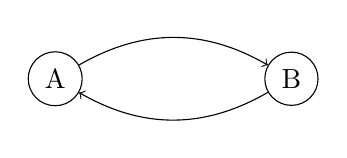
\begin{tikzpicture}
            \node[circle, draw] (A) at (0,0) {A};
            \node[circle, draw] (B) at (3,0) {B};
            \draw[->] (A) to[bend left] (B);
            \draw[->] (B) to[bend left] (A);
        \end{tikzpicture}
    \end{center}
\end{frame}

\begin{frame}{Arten von Kausalität: Gemeinsamer Grund}
    \textbf{Gemeinsamer Grund} beschreibt eine Situation, in der eine dritte Variable sowohl A als auch B beeinflusst. Zum Beispiel könnte C sowohl A als auch B beeinflussen.
    \begin{center}
        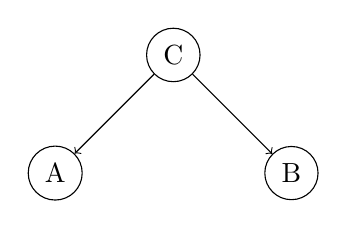
\begin{tikzpicture}
            \node[circle, draw] (C) at (1.5,1.5) {C};
            \node[circle, draw] (A) at (0,0) {A};
            \node[circle, draw] (B) at (3,0) {B};
            \draw[->] (C) -- (A);
            \draw[->] (C) -- (B);
        \end{tikzpicture}
    \end{center}
\end{frame}

\begin{frame}{Arten von Kausalität: Indirekte Kausalität}
    \textbf{Indirekte Kausalität} beschreibt eine Situation, in der A B beeinflusst, aber nicht direkt. Zum Beispiel könnte A C beeinflussen und C B beeinflussen.
    \begin{center}
        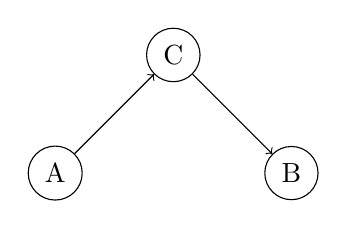
\begin{tikzpicture}
            \node[circle, draw] (A) at (0,0) {A};
            \node[circle, draw] (C) at (1.5,1.5) {C};
            \node[circle, draw] (B) at (3,0) {B};
            \draw[->] (A) -- (C);
            \draw[->] (C) -- (B);
        \end{tikzpicture}
    \end{center}
\end{frame}

\begin{frame}{Arten von Kausalität: Direkte Kausalität}
    \textbf{Direkte Kausalität} beschreibt eine Situation, in der A B direkt beeinflusst. Zum Beispiel könnte A B beeinflussen, ohne dass eine dritte Variable dazwischen steht.
    \begin{center}
        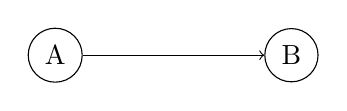
\begin{tikzpicture}
            \node[circle, draw] (A) at (0,0) {A};
            \node[circle, draw] (B) at (3,0) {B};
            \draw[->] (A) -- (B);
        \end{tikzpicture}
    \end{center}
\end{frame}

\begin{frame}[fragile]{Auftrag}
    \begin{itemize}
        \item \aufgabebox{1.2 im Skript}
    \end{itemize}
\end{frame}

\begin{frame}{Lösung: Korrelation oder Kausalität? (1)}
    \textbf{Lösung:} \textbf{Koinzidenz}: Keine kausale Beeinflussung. Die Korrelation ist zufällig oder durch eine Drittvariable erklärbar (z.B. mehr Stress $\rightarrow$ mehr Kaffee).
    \begin{center}
        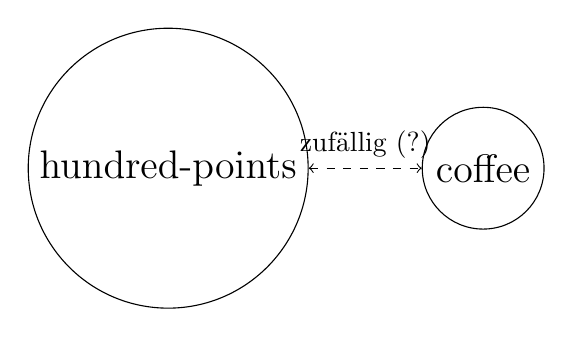
\begin{tikzpicture}
            \node[circle, draw] (A) at (0,0) {\Large\emoji{hundred-points}};
            \node[circle, draw] (B) at (4,0) {\Large\emoji{coffee}};
            \draw[<->, dashed] (A) -- (B) node[midway, above] {zufällig (?)};
        \end{tikzpicture}
    \end{center}
\end{frame}

\begin{frame}{Lösung: Korrelation oder Kausalität? (2)}
    \textbf{Lösung:} \textbf{Gemeinsamer Grund}: Beide Grössen werden durch eine Drittvariable beeinflusst: das Wetter bzw. die Jahreszeit.
    \begin{center}
        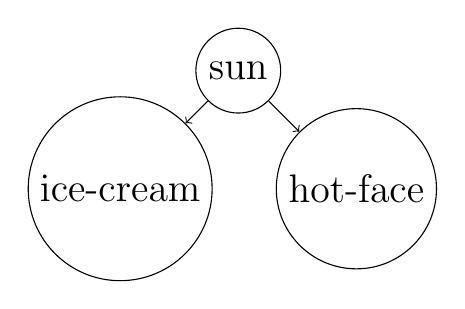
\begin{tikzpicture}
            \node[circle, draw] (C) at (1.5,1.5) {\Large\emoji{sun}};
            \node[circle, draw] (A) at (0,0) {\Large\emoji{ice-cream}};
            \node[circle, draw] (B) at (3,0) {\Large\emoji{hot-face}};
            \draw[->] (C) -- (A);
            \draw[->] (C) -- (B);
        \end{tikzpicture}
    \end{center}
\end{frame}

\begin{frame}{Lösung: Korrelation oder Kausalität? (3)}
    \textbf{Lösung:} \textbf{Koinzidenz}: Keine echte Beeinflussung. Es handelt sich um eine Scheinkorrelation ohne sinnvollen Zusammenhang.
    \begin{center}
        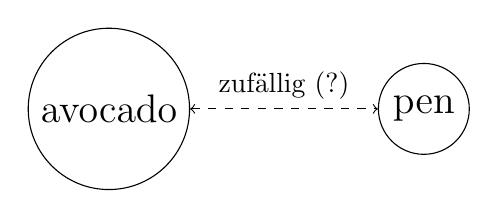
\begin{tikzpicture}
            \node[circle, draw] (A) at (0,0) {\Large\emoji{avocado}};
            \node[circle, draw] (B) at (4,0) {\Large\emoji{pen}};
            \draw[<->, dashed] (A) -- (B) node[midway, above] {zufällig (?)};
        \end{tikzpicture}
    \end{center}
\end{frame}

\begin{frame}{Lösung: Korrelation oder Kausalität? (4)}
    \textbf{Lösung:} \textbf{Indirekte Kausalität}: SportlerInnen schlafen besser, was zu besseren Prüfungsergebnissen führt.
    \begin{center}
        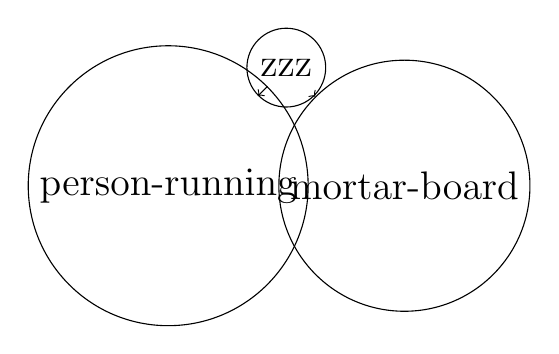
\begin{tikzpicture}
            \node[circle, draw] (A) at (0,0) {\Large\emoji{person-running}};
            \node[circle, draw] (C) at (1.5,1.5) {\Large\emoji{zzz}};
            \node[circle, draw] (B) at (3,0) {\Large\emoji{mortar-board}};
            \draw[->] (A) -- (C);
            \draw[->] (C) -- (B);
        \end{tikzpicture}
    \end{center}
\end{frame}

\begin{frame}{Lösung: Korrelation oder Kausalität? (5)}
    \textbf{Lösung:} \textbf{Zyklische Beeinflussung}: Stress führt zu schlechteren Noten, was wiederum zu mehr Stress führt.
    \begin{center}
        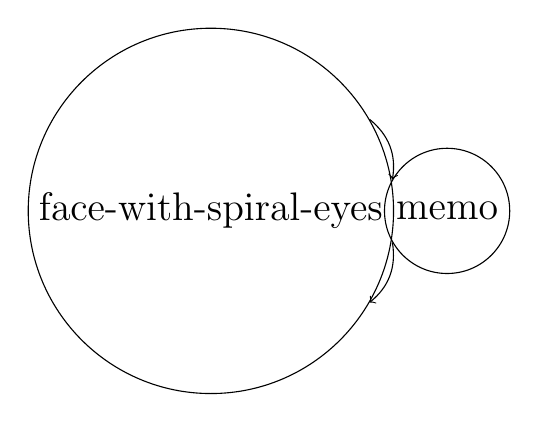
\begin{tikzpicture}
            \node[circle, draw] (A) at (0,0) {\Large\emoji{face-with-spiral-eyes}};
            \node[circle, draw] (B) at (3,0) {\Large\emoji{memo}};
            \draw[->] (A) to[bend left] (B);
            \draw[->] (B) to[bend left] (A);
        \end{tikzpicture}
    \end{center}
\end{frame}

\begin{frame}{Korrelations-Beispiel: Abweichung vom Mittelwert}
    \begin{figure}[H]
        \centering
        \begin{subfigure}[t]{0.48\textwidth}
            \centering
            \includegraphics[width=\linewidth]{"GrundlagenInfo/10_AusDatenLernen/Figures/polizei_vs_kriminalitaet"}
            \caption{Ursprüngliche Daten}
            \label{fig:polizei_vs_kriminalitaet}
        \end{subfigure}
        ~
        \begin{subfigure}[t]{0.48\textwidth}
            \centering
            \includegraphics[width=\linewidth]{"GrundlagenInfo/10_AusDatenLernen/Figures/polizei_vs_kriminalitaet_correl"}
            \caption{Daten als Abweichung vom Mittelwert}
            \label{fig:socialmedia_vs_zufriedenheit}
        \end{subfigure}
    \end{figure}
    \[
        Z = x_1' \cdot y_1' + x_2' \cdot y_2' + \dots + x_n' \cdot y_n'
    \]
    \begin{itemize}
        \item \( x_i' \): Abweichung der Variable \(x\) vom Mittelwert
        \item \( y_i' \): Abweichung der Variable \(y\) vom Mittelwert
    \end{itemize}
\end{frame}

\begin{frame}[fragile]{Auftrag}
    \begin{itemize}
        \item \aufgabebox{1.3 im Skript, mit Excel \faFileExcel{}}
    \end{itemize}
\end{frame}